\documentclass[output=paper]{langscibook}
\ChapterDOI{10.5281/zenodo.4729789}

\author{Sacha Beniamine\affiliation{Department of Linguistic and Cultural Evolution, Max Planck Institute EVA}}
\title{One lexeme, many classes: Inflection class systems as lattices}

\abstract{This paper discusses the nature of inflection classes (ICs) and provides a fully implemented methodology to conduct typological investigations into their structure.

	ICs (conjugations or declensions) are sets of lexemes which inflect similarly. They are often described as partitioning the set of lexemes, but similarities across classes lead some authors to favor hierarchical
	descriptions. While some formalisms allow for multiple inheritance, where one class takes after two or more others, it is usually taken as an exceptional situation.

	I submit that the structure of ICs is a typological property of inflectional systems. As a result, ICs are best modelled as semi-lattices, which  by design capture non-canonical phenomena. I show how these monotonous multiple inheritance hierarchies can be inferred automatically from raw paradigms using alternation patterns and formal concept analysis. Using quantitative measures of canonicity, I compare six inflectional systems and show that multiple inheritance is in fact pervasive across inflectional systems.}


\begin{document}
\maketitle

    \section{Introduction}
    \label{Introduction:beniamine}

    In some inflectional systems, the same morphosyntactic properties can be expressed differently across lexemes. Descriptions of the resulting inflection classes (declensions or conjugations) can take several forms. The simplest possibility is to use a partition of the set of lexemes into classes, as in Figure~\ref{fig:beniamine:models}a. Possible partitions will differ in their granularities. Pedagogical grammars are often content with giving a broad classification in major classes. At the other end of the spectrum, various studies (e.g. \citealt{StumpFinkel2013}) presuppose a classification into numerous fine-grained classes.

    \begin{figure}
        \begin{tabular}{cccc}
            %        \lsptoprule
            a. Partition & b.  Tree & c. Semi-lattice \\
            %        \midrule
            \includegraphics{figures/partition.pdf}&
            \includegraphics{figures/tree-small.pdf}&
            \includegraphics{figures/lattice.pdf}\\
            %        \lspbottomrule
        \end{tabular}
        \caption{Three types of classification structures}
        \label{fig:beniamine:models}
    \end{figure}

    Broad and fine-grained classifications can be linked by assuming
    a hierarchic\-ally-organized system of classes
    \citep{CorbettFraser1993,DresslerThornton1996}. In recent years,
    various efforts have been made towards inferring inflection class
    hierarchies automatically from paradigms
    \citep{BrownHippisley2012,LeeGoldsmith2013,Bonamihdr}. While they
    use very different methodologies, most of these approaches
    converge on the use of tree-shaped hierarchies
    (Figure~\ref{fig:beniamine:models}b.). Network morphology
    \citep{CorbettFraser1993,BrownHippisley2012} uses richer structure
    through default inheritance and multiple inheritance of orthogonal
    properties, but does not allow for multiple inheritance in a
    single dimension (e.g. affixes).

    In this paper, I argue that while ``inflection classes'' (IC) usually refers to either partitions (Figure~\ref{fig:beniamine:models}a.) or trees (Figure~\ref{fig:beniamine:models}b.), these make simplifications which overlook numerous relations between lexemes and hide structural properties that are in fact pervasive. I show that semi-lattices (Figure~\ref{fig:beniamine:models}c.), where one subclass may belong to more than one superclass, are more faithful models of inflectional systems. I use formal concept analysis (\citealt{GanterWille1998}, hereafter FCA) to automatically infer semi-lattices of inflection classes for the verbal systems of French, English, Modern Standard Arabic, European Portuguese and Zenzontepec Chatino; as well as for the nominal system of Russian.\footnote{The methodology described in this paper is fully implemented as part of the Qumín toolkit \citep{BeniaminePhd} which can be accessed at: \url{https://github.com/XachaB/Qumin}. Qumín is distributed under GPLv.3.}

    I compare these systems using canonical typology. To do so, I provide formal definitions of inflectional structure and precise quantitative measures of inflectional canonicity, which can be computed automatically from a large inflected lexicon.

	Inflection classes are usually taken as classes of lexemes or stems related by common affixes \citep{Carstairs1987,Carstairs-McCarthy1991,StumpFinkel2013}. However, alternations between stems also contribute to the expression of inflectional information. Segmentation in stems and affixes is useful to produce systems in constructive approaches \citep[in the sense of][]{Blevins2006}, where the goal is to generate the forms from a minimal grammar. Instead, I adopt here the abstractive approach \citep{Blevins2006} and attempt to account for all interesting generalizations. As a consequence, I take \textsc{inflectional behavior} to be relations between word-forms, or \textsc{alternation patterns}, rather than affixes \citep{BonamiLuis2014, BonamiBeniamine2016}.

    In the first section, I present partition- and tree-based accounts of ICs. Next, I motivate the need for multiple inheritance hierarchies as a more truthful model of ICs. In Section 3, I present FCA, which can be used to infer a semi-lattice of classes. The last section contrasts the properties of the IC lattices of six languages.

\section{The structure of inflection class systems}
    \label{Section:beniamine:structure-of-IC-systems}

    IC systems are often described as a partition of a few broad classes of lexemes which share some of their inflectional behavior. Partitions of ICs are used both in pedagogical grammars and in many descriptive accounts. They usually count only a few classes. They are, as \citet[129]{Matthews1991} puts it, ``classes of lexemes that go together in respect of some inflection''. This definition relies on the inflectional similarity between lexemes.

    \citet{Corbett1982} counts six nominal ICs (declensions) in Russian, which Table~\ref{tab:beniamine:CorbettRusN} illustrates by showing the full paradigm of one exemplar lexeme per class. I indicate frequencies based on counts in a lexicon of 1,239 nouns \citep{BeniamineBrown2019} described in more detail in the appendix and in \cite{BeniaminePhd}.
    % \citet{BeniaminePhd}'s lexicon of russian nouns, which comprises 1539 nouns.

    \begin{table}
      \tabcolsep.9\tabcolsep %%% BC: This is intentional!
        \begin{tabular}{+l^l^l^l^l^l^l}
            \lsptoprule
            	\textup{lexeme}           & \mysc zakon & \mysc vino & \mysc škola   & \mysc kost' & \mysc put' & \mysc vremja \\
            \midrule
            gloss            & `law'     & `wine'   &  `school'   & `bone'    &  `way'   & `time' \\
            frequency        & 874       & 96       &    428      & 112       &    1     &    6      \\
            \midrule
            \unitrow
            \textsc{\upshape{nom.sg}}  &\gry[0.7]zakon     &  vino    &\gry  škola      &\gry[0.7]  kost'    &\gry[0.7]  put'    &\gry vremja    \\
            \unitrow
            \textsc{\upshape{acc.sg}}  &\gry[0.7]zakon     &  vino    &  školu      &\gry[0.7]  kost'    &\gry[0.7]  put'    & vremja    \\
            \unitrow
            \textsc{\upshape{gen.sg}}  &\gry zakona    &\gry  vina    &  školy      &\gry[0.7]  kosti    &\gry[0.7]  puti    &\gry[0.7] vremeni    \\
            \unitrow
            \textsc{\upshape{dat.sg}}  & zakonu    &  vinu    &  škole      &\gry[0.7]  kosti    &\gry[0.7]  puti    &\gry[0.7] vremeni    \\
            \unitrow
            \textsc{\upshape{ins.sg}} &\gry zakonom   &\gry  vinom   &  školoj     &  kost'ju  &\gry[0.7]  putem    &\gry[0.7] vremenem    \\
            \unitrow
            \textsc{\upshape{loc.sg}}  &\gry zakone    &\gry  vine    &\gry  škole      &\gry[0.7]  kosti    &\gry[0.7]  puti    &\gry[0.7] vremeni    \\
            \unitrow
            \textsc{\upshape{nom.pl}}  &\gry zakony    &  vina    &\gry  školy      &\gry[0.7]  kosti    &\gry[0.7]  puti    & vremena    \\
            \unitrow
            \textsc{\upshape{acc.pl}}  &\gry zakony    &  vina    &\gry  školy      &\gry[0.7]  kosti    &\gry[0.7]  puti    & vremena    \\
            \unitrow
            \textsc{\upshape{gen.pl}}  & zakonov   &\gry  vin     &\gry  škol       &\gry[0.7]  kostej   &\gry[0.7] putej    & vremen    \\
            \unitrow
            \textsc{\upshape{dat.pl}}  &\gry zakonam   &\gry  vinam   &\gry  školam     &\gry  kostjam  &\gry putjam    &\gry vremenam    \\
            \unitrow
            \textsc{\upshape{ins.pl}} &\gry zakonami  &\gry  vinami  &\gry  školami    &\gry  kostjami &\gry putjami    &\gry vremenami    \\
            \unitrow
            \textsc{\upshape{loc.pl}}  &\gry zakonax   &\gry  vinax   &\gry  školax     &\gry  kostjax  &\gry putjax    &\gry vremenax    \\

            \lspbottomrule
        \end{tabular}
        %
        %    irreg       1
        %    invar      21

        \caption{Six broad inflection classes of Russian in Roman transliteration, according to~\citet[203]{Corbett1982} }
        \label{tab:beniamine:CorbettRusN}
    \end{table}

    While it is usually thought that there is only one correct inventory of ICs in a given system, the number of classes is in fact often disputed, even in very well-documented languages. \citet[202]{Corbett1982} highlights such disagreements in the case of Russian nouns: ``The reader not familiar with the literature will quite reasonably expect a straightforward account of the paradigms in Russian. Tradition answers three, some writers claim four, and more recently it has been suggested that only two paradigms are required''. The situation of Russian nouns is far from exceptional. One reason is that constructive and pedagogical analyses both usually strive for the shortest possible description. This leads to the merging of classes wherever possible, for example where distinct surface realizations can be abstracted away as allomorphy or predicted using semantic or grammatical properties of the lexemes. For example, Corbett shows that most descriptions of the ICs of Russian nouns merge together the classes \textsc{zakon} and \textsc{vino}. The classes \textsc{kost'} and \textsc{put'} are also usually merged, sometimes with the class \textsc{vremja}. In a similar fashion, \citet{Plenat87} provides a two-class analysis of the French verbal inflectional system, which is usually described as having three conjugations. To do so, he merges the second and third conjugation using abstract phonological representations. \citet{Blevins2004} reports that the nominal system of Estonian has been described as having between 26 and 400 ``paradigms'', which can be merged in 6 to 12 ICs.\largerpage

    Going back to the data presented in Table~\ref{tab:beniamine:CorbettRusN}, two shades of gray indicate some similarities across classes in each cell. All the classes share realizations for the dative, instrumental and locative plural. The class \textsc{zakon} shares the same endings as the class \textsc{vino} for the genitive, instrumental and locative singular. The locative singular is also identical to that of \textsc{škola}. \textsc{zakon} and \textsc{škola} also share the same endings in the nominative and accusative plural, while \textsc{vino} and \textsc{škola} both present no affixes in the genitive plural. The nominative and accusative singular of \textsc{zakon}, like those of \textsc{kost'} and \textsc{put'}, show no affixes on the stem, etc. To these similarities in terms of endings or affixes, one could add similarities in terms of alternations, such as syncretisms: for example, the classes \textsc{zakon}, \textsc{vino}, \textsc{kost'}, \textsc{put'} and \textsc{vremja} (but not \textsc{škola}) all present a syncretism between nominative and accusative singular. All these lexemes share a syncretism between the nominative and accusative plural.

    A look at the Russian lexicon described in the appendix shows that the behavior of lexemes inside each class is less homogeneous than suggested by the table of exemplars. While all the exemplars shown above are inanimate and present the accusative-nominative syncretism, I found several lexemes with an accusative-genitive syncretism (typical of animates): 163 in the class \textsc{zakon}, 8 in the class \textsc{vino}, 47 in the class \textsc{škola} and 6 in the class \textsc{kost'} \citep[see][129]{CorbettFraser1993}. Moreover, 76 lexemes of the class \textsc{zakon}, 3 of the class \textsc{vino} and 6 of the class \textsc{škola} have genitives in \unit{-ej} rather than \unit{-ov} or the bare stem.

    Since similarity is gradient, it is difficult to determine how similar lexemes need to be to belong to the same class. Recent works in computational linguistics have attempted to decide on the best partition using minimal description length, either by comparing hand-written analysis \citep{WaltherSagot2011} or by generating the analysis automatically from the data \citep{BeniamineBonamiSagot2017}. But even when selected very rigorously, the resulting partitions are simplifications. They can be useful as pedagogical tools, or as compact constructive descriptions, but they do not account for all similarities between classes, nor for the internal variation in each class.

    At the other end of the descriptive spectrum, various studies take ICs as very fine-grained partitions, where each distinction in inflectional behavior warrants a separate class. IC membership is then defined in terms of identity. \citet[64]{Aronoff1994} defines an IC as ``a set of lexemes whose members each select the same set of inflectional realizations''. \citet[739]{Carstairs-McCarthy1994} provides two definitions of a paradigm:

    \blockquote{%
        (1) \textsc{paradigm$_{1}$}: the set of combinations of morphosyntactic properties or features (or the set of ``cells'') realized by inflected forms of words (or lexemes) in a given word-class (or major category or lexeme-class) in a given language.\\
        (2) \textsc{paradigm$_{2}$}: the set of inflectional realizations expressing a paradigm$_{1}$ for a given word (or lexeme) in a given language.
    }

    Based on these definitions, he offers a very similar definition of ICs: ``a set of words (lexemes) displaying the same paradigm$_{2}$ in a given language''. Applied to realistic datasets, these definitions yield a high number of classes, many of which are often very small. \citet{StumpFinkel2013} report 72 ICs for French verbs, while \citet{Bonamihdr}, \citet{BeniamineBonamiSagot2017} and \citet{BeniaminePhd} find up to 97 classes.\footnote{While they all base their computations on the Flexique lexicon \citep{BonamiCaronPlancq2014}, differences across accounts are due both to different methodologies and to corrections that have been made in the lexicon since its publication.} For Russian nouns, \citet{BeniaminePhd} identifies 159 ICs based on identity of surface segmental inflectional behavior (not counting stress patterns). While, by definition, these classes do not show any internal heterogeneity, enumerating them does not account for any similarities across classes.

    Descriptive grammars often make use of explicit or implicit tree-shaped hierarchies when they provide several granularity levels. For example, the French pedagogical grammar Bescherelle \citep{bescherelle} describes three ICs, each exemplified by numerous verbal exemplars (one per page) and finer variations in footnotes. These can be interpreted as a three-level hierarchy. \citet{Campbell2011} describes the ICs in Zenzontepec Chatino, an Oto-Manguean language spoken in Oaxaca, by a three-level hierarchy presented in Figure~\ref{fig:beniamine:czntree}. Zenzontepec Chatino expresses inflection through prefixes and has only four paradigm cells: potential, habitual, progressive and completive. Figure~\ref{fig:beniamine:czntree} shows common prefixes for each node of the hierarchy. The notation ``[lam]'' marks the laminalization of initial \unitup{[t]} in class Bt. \citet{Campbell2011} shows identical underlying prefixes for classes Au and Ac, but they differ on the surface. Class Bc presents a stem-initial alternation between \unit{y-} and \unit{ch-}. Since class C2 presents several distinct affixes, it could be further divided in two distinct classes. The first level of \citets{Campbell2011} classification is not based on similarity alone, but inherits from \citets{Kaufman1989} description of Zapotec ICs.

    \begin{figure}
        \begin{tikzpicture}[baseline={(current bounding box.north)},grow'=right]
        \tikzset{level distance=95pt}
        \tikzset{every tree node/.style={align=center,anchor=west}}
        \Tree[.{} [.{A\\\smaller\begin{tabular}{l>{\unitfamily}l}%
            \textsc{prog} & \unit{nte-}  \\%
            \end{tabular}} [.{Au/Ac\\\smaller\begin{tabular}{l>{\unitfamily}l}%
            \textsc{comp} & \unit{nka-}  \\%
            \end{tabular}} [.{Au\\\smaller\begin{tabular}{l>{\unitfamily}l}%
            \textsc{pot} & \unit{ku-}  \\%
            \textsc{hab} & \unit{ntu-}  \\%
            \end{tabular}} ] [.{Ac\\\smaller\begin{tabular}{l>{\unitfamily}l}%
            \textsc{pot} & \unit{ki-}  \\%
            \textsc{hab} & \unit{nti-}  \\%
            \end{tabular}} ] ] [.{A2\\\smaller\begin{tabular}{l>{\unitfamily}l}%
            \textsc{pot} & \unit{ki-}  \\%
            \textsc{hab} & \unit{nti-}  \\%
            \textsc{comp} & \unit{nkwi-}  \\%
            \end{tabular}} ] ] [.{B\\\smaller\begin{tabular}{l>{\unitfamily}l}%
            \textsc{prog} & \unit{nte-}  \\%
            \textsc{comp} & \unit{nk}(\unit{u})\unit{-}  \\%
            \end{tabular}} [.{Bc\\\smaller\begin{tabular}{l>{\unitfamily}l}%
            \textsc{pot} & \unit{ki-}  \\%
            \textsc{hab} & \unit{nti-}  \\%
            \end{tabular}} ] [.{Bt\\\smaller\begin{tabular}{l>{\unitfamily}l}%
            \textsc{pot} & [lam]  \\%
            \textsc{hab} & \unit{n-} [lam]  \\%
            \end{tabular}} ] [.{Bc\\\smaller\begin{tabular}{l>{\unitfamily}l}%
            \textsc{pot} & stem \unit{y-} $\to$ \unit{ch-} \\%
            \textsc{hab} & \unit{n-} stem \unit{y-} $\to$ \unit{ch-}  \\%
            \end{tabular}} ] ] [.{C\\    \smaller\begin{tabular}{l>{\unitfamily}l}%
            \textsc{pot} & \unit{k-}  \\%
            \textsc{hab} & \unit{nti-}  \\%
            \end{tabular}} [.{Ca\\      \smaller\begin{tabular}{l>{\unitfamily}l}%
            \textsc{prog} & \unit{nch-}  \\%
            \textsc{comp} & \unit{nku-}  \\%
            \end{tabular}} ] [.{C2\\      \smaller\begin{tabular}{l>{\unitfamily}l}%
            \textsc{prog} & \unit{ntey-},\unit{nch-}  \\%
            \textsc{comp} & \unit{nkay-},  \unit{y-}  \\%
            \end{tabular}} ] ] ]

        \end{tikzpicture}
        \caption{Inflection class tree in Zenzontepec Chatino verbs according to \citet[229]{Campbell2011}}
        \label{fig:beniamine:czntree}
    \end{figure}

    \citet{DresslerThornton1996}, \citet{Kilani-SchochDressler2005} and \citet{DresslerKilani-SchochGagarinaPestalPoechtrager2008} use the term ``macroclass'' for the broad ICs based on similarity and ``microclass'' for the fine-grained ICs based on identity of inflectional behavior. They link both in tree-shaped hierarchies, in which any node can be seen as an IC. Microclasses form the leaves of the hierarchy, while macroclasses form the first level below the root. Any number of intermediate classes is possible. In \citets{Kilani-SchochDressler2005} approach to French, the macroclasses are not based on similarity alone, but instead they constitute a bipartition between productive and unproductive patterns. Each IC is motivated by common inflectional patterns, written as implicative statements which the authors call ``paradigm structure conditions''. These conditions are inherited by default.

    In network morphology \citep{CorbettFraser1993,BrownHippisley2012}, ICs are also represented by a tree-shaped default inheritance hierarchy. The analyses are constructive: couched in the \textsc{datr} formalism, each node specifies affixal rules. The grammar is designed to generate surface forms. Default inheritance has two main advantages. First, it allows for more compact representations by limiting repetitions and the overall number of nodes in the hierarchy. Second, it gives the notion of regularity a natural status: a node which rewrites a default is exceptional relative to the ancestor which stipulated the default rule.

    \begin{sloppypar}
    Going back to Russian nouns, \citet{Brown1998} count four main ICs which correspond to the first four declensions described by \citet{Corbett1982}:
    \textsc{zakon} (I), \textsc{škola}~(II), \textsc{kost'} (III) and  \textsc{vino} (IV). \citet{Brown1998} argues in favor of the hierarchical structure summarized in Figure~\ref{fig:beniamine:BrownRusN}. In the inflectional tree, the leaves \textsc{n\_i} to \mbox{\textsc{n\_iv}} stand for each of the four ICs. The root is the node \textsc{mor\_nominal}, which also spans adjectives (which I will ignore for the purpose of this paper). It defines common properties between nouns and adjectives, as well as two default values: a zero affix in the nominative singular and an \unit{-i} ending in the nominative plural. The term \textsc{evaluation} denotes the usage of a realization function which takes as input morphological properties of a lexeme and can assign distinct values to lexemes belonging to the same class. The node \textsc{mor\_nom} specifies a thematic vowel characteristic of all nouns, a default affixal value for the locative singular and a default syncretism between dative and locative singular. There is only one intermediate node, \textsc{n\_o}. It manifests properties shared between classes~I and~IV.
    \end{sloppypar}

    \begin{figure}
        \renewcommand{\arraystretch}{0.8}
        \resizebox{\linewidth}{!}{%
            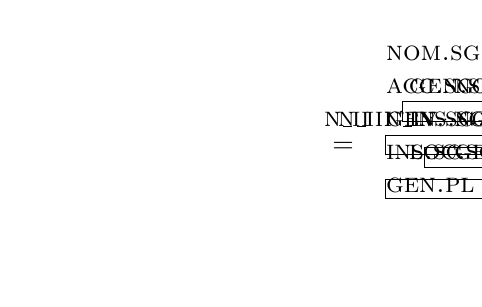
\begin{tikzpicture}[baseline={(current bounding box.north)}]
            \tikzset{level distance=85pt}
            \tikzset{every tree node/.style={align=center,anchor=north}}
            \Tree[.{\textsc{mor\_nominal}\\%
                \smaller \begin{tabular}{l>{\unitfamily\itshape}l} %
                \textsc{nom.sg} & --- \\%
                \textsc{acc.sg} & \myrm \textsc{evaluation} \\%
                \textsc{nom.pl} & -i \\%
                \textsc{acc.pl} & \myrm \textsc{evaluation} \\%
                \textsc{dat.pl} & -m \\%
                \textsc{ins.pl} & -mi \\%
                \textsc{loc.pl} & x \\%
                \end{tabular}} %
            [.{\textsc{mor\_adjective}\\...} ] [.{\textsc{mor\_noun}\\%
                \smaller \begin{tabular}{l>{\unitfamily\itshape}l} %
                {\smaller thematic vowel} & -a- \\%
                \textsc{loc.sg} & -e \\%
                \textsc{dat.sg} & $=$  \myrm\textsc{loc.sg} \\%
                \end{tabular}} [.{\textsc{n\_o}\\%
                \smaller \begin{tabular}{l>{\unitfamily\itshape}l} %
                \textsc{gen.sg} & -a \\%
                \textsc{dat.sg} & -u \\%
                \textsc{ins.sg} & -om \\%
                \end{tabular}} [.{\textsc{n\_I}\\%
                \smaller \begin{tabular}{l>{\unitfamily\itshape}l}%
                \textsc{gen.pl} & -ov \\%
                \end{tabular}} ] \node(ref1){\textsc{n\_iv}\\%
                \smaller \begin{tabular}{l>{\unitfamily\itshape}l} %
                \textsc{nom.sg} & -o \\%
                %\textsc{acc.sg} & -o \\%
                \textsc{nom.pl} & -a \\%
                %\textsc{acc.pl} & -a \\%
                \textsc{gen.pl} &  \\%
                \end{tabular}};  ]  \node(ref2){\textsc{n\_ii}\\%
                \smaller \begin{tabular}{l>{\unitfamily\itshape}l}%
                \textsc{nom.sg} & -a \\%
                \textsc{acc.sg} & -u \\%
                \textsc{gen.sg} & -i  \\%
                \textsc{ins.sg} & -oj(u) \\%
                \textsc{gen.pl} & \myrm \textsc{evaluation}\\%
                \end{tabular}}; \node(ref3){\textsc{n\_iii}\\%
                \smaller \begin{tabular}{l>{\unitfamily\itshape}l}%
                \textsc{gen.sg} &  \\%
                \textsc{ins.sg} & -ju \\%
                \textsc{loc.sg} & $=$ \myrm \textsc{gen.sg} \\%
                \end{tabular}};   ] ] ]

            \node[draw,minimum width=2cm,inner sep=3.5pt] (IV) at ([yshift=0.8em]ref1.south){};
            \node[draw,minimum width=3cm,inner sep=3.5pt] (IIGENPL) at ([yshift=0.85em]ref2.south){};
            \node[draw,minimum width=3cm,inner sep=3.5pt] (IIGENSG) at ([yshift=5.7ex]ref2.south){};
            \node[draw,minimum width=2cm,inner sep=3.5pt] (IIIGENSG) at ([yshift=5.7ex,xshift=-0.8em]ref3.south){};

            \draw[semithick,dotted,->] (IV.east) .. controls +(east:2) and +(south:1).. (IIGENPL.south);
            \draw[semithick,dotted,->] (IIIGENSG.west) .. controls +(west:.5) and +(east:.5).. (IIGENSG.east);
            \end{tikzpicture}}
        \caption{\textsc{datr} hierarchy for Russian nouns according to \citet[Theory B, ~128 et seq.]{Brown1998}}
        \label{fig:beniamine:BrownRusN}
    \end{figure}

    In \citets{Brown1998} account, some commonalities between classes are not modeled through the tree structure itself but by direct references across classes for specific cells. These references are indicated in Figure~\ref{fig:beniamine:BrownRusN} by dotted arcs between framed cells. For example, the genitive plural of class IV is formed by using the evaluation functions of the genitive plural in class II. The need for this second mechanism highlights the inadequacy of a tree structure to express all similarities between ICs. In addition, while default inheritance is useful for producing a compact hierarchy, it hides the exact span of the default rules. In the following section, I show how a richer hierarchy can account more naturally for IC structure in an abstractive approach.

    %Several studies have recently contributed to automatical inference of tree-shaped hierarchies from full form paradigms. For example, \citet{BrownEvans2012} validate \citet{Brown1998}'s theory by generating a tree which minimizes compression distances between whole forms. \citet{Bonamihdr} produces distance based trees over French paradigms using agglomerative clustering (UPGMA). \citet{LeeGoldsmith} try to infer tree hierarchies for Greek nouns and English verbs using description length.

    \FloatBarrier

    \section{Noncanonical systems as inflection class lattices}
    \label{Section:non-canonical-systems-as-inflectional-lattices}

    In the previous section, I showed that partitions and tree structures have been used to describe inflectional systems even when their similarity structure is more complex than these descriptive devices can account for. It is, however, conceivable that some inflectional systems do conform to the structure of either a partition or a tree.
    % \cite[63]{Wurzel1989} describes as follows the properties of an ideal system of inflection classes: ``The constitution of inflectional classes is based on the uniformity and distinctiveness of paradigms, just as every classification is based on the common and distinct properties of the elements to be classified''.

    \citet{Corbett2009} chooses this particular ideal structure as a canonical point of comparison for typological investigation. He defines canonical IC systems as following the principle of distinctiveness \citep[3]{Corbett2009}, which can be evaluated using four criteria:

    \begin{quote}
        PRINCIPLE I (distinctiveness): Canonical inflection classes are fully comparable and are distinguished as clearly as is possible.
        [...]
        \begin{description}
            \item[criterion 1] In the canonical situation, forms differ as consistently as possible across
            inflectional classes, cell by cell.
            \item[criterion 2] Canonical inflectional classes realize the same morphosyntactic or
            morphosemantic distinctions (they are of the same structure).
            \item[criterion 3] Within a canonical inflectional class each member behaves identically.
            \item[criterion 4] Within a canonical inflectional class each paradigm cell is of equal status.
        \end{description}
    \end{quote}

    From these criteria, it follows that in a canonical system, there are no similarities between classes. If two classes were to have a common exponent or alternation pattern, they would violate criterion~1. Moreover, the cells affected by common patterns would then be less predictive of the ICs than other cells, which violates criterion~4. According to criterion~2, a canonical system of ICs can have only one form per paradigm cell and lexeme. Defective lexemes, which lack forms for certain cells and overabundant lexemes, which have more than one possible form for certain cells, violate criterion~2. Finally, criterion~3 means that all classes are microclasses: they are based on identity. In a canonical system, micro- and macroclasses coincide. The system then truly has the shape of a partition (or a one-level tree, with classes as leaves and the whole system as root).

    If real systems mostly conformed to the canonical ideal -- which is not usually expected -- then it would be adequate to model them using partitions. If, however, noncanonicity is the norm, then more expressive models are required. Since partitions and trees make the assumption of a certain degree of canonicity, these models are not suited to evaluating a system's position in the canonical space.

    Figure~\ref{fig:beniamine:RusPartition} shows the same four ICs of Russian nouns as in Figure~\ref{fig:beniamine:BrownRusN}, now arranged as a partition, with each class characterized by affixes. While the shape of this classification is that of a partition, it is obvious from the numerous repetitions that it is not the structure of the data. The use of a partition masks the system's noncanonicity.

    \begin{figure}
        \renewcommand{\arraystretch}{0.8}
        \resizebox{\linewidth}{!}{
            \begin{tikzpicture}[baseline={(current bounding box)}]
            \tikzset{level distance=40pt,sibling distance=20pt}
            \tikzset{every tree node/.style={align=center,anchor=north}}
            \Tree[.{\textsc{}\\%
                \smaller } [.{\textsc{n\_i}\\%
                \smaller \begin{tabular}{l>{\unitfamily\itshape}l}%
                \textsc{nom.sg} & --- \\%
                \textsc{acc.sg} & --- \\%
                \textsc{gen.sg} & -a \\%
                \textsc{dat.sg} & -u \\%
                \textsc{ins.sg} & -om \\%
                \textsc{prep.sg} & -e \\%
                \textsc{nom.pl} & -i \\%
                \textsc{acc.pl} & -i \\%
                \textsc{gen.pl} & -ov \\%
                \textsc{dat.pl} & -am \\%
                \textsc{ins.pl} & -ami \\%
                \textsc{prep.pl} & -ax \\%
                \end{tabular}} ] [.{\textsc{n\_iv}\\%
                \smaller \begin{tabular}{l>{\unitfamily\itshape}l} %
                \textsc{nom.sg} & -o \\%
                \textsc{acc.sg} & -o \\%
                \textsc{gen.sg} & -a \\%
                \textsc{dat.sg} & -u \\%
                \textsc{ins.sg} & -om \\%
                \textsc{prep.sg} & -e \\%
                \textsc{nom.pl} & -a \\%
                \textsc{acc.pl} & -a \\%
                \textsc{gen.pl} & --- \\%
                \textsc{dat.pl} & -am \\%
                \textsc{ins.pl} & -ami \\%
                \textsc{prep.pl} & -ax \\%
                \end{tabular}} ]  [.{\textsc{n\_ii}\\%
                \smaller \begin{tabular}{l>{\unitfamily\itshape}l}%
                \textsc{nom.sg} & -a \\%
                \textsc{acc.sg} & -u \\%
                \textsc{gen.sg} & -i \\%
                \textsc{dat.sg} & -e \\%
                \textsc{ins.sg} & -oj \\%
                \textsc{prep.sg} & -e \\%
                \textsc{nom.pl} & -i \\%
                \textsc{acc.pl} & -i \\%
                \textsc{gen.pl} & --- \\%
                \textsc{dat.pl} & -am \\%
                \textsc{ins.pl} & -ami \\%
                \textsc{prep.pl} & -ax \\%
                \end{tabular}} ] [.{\textsc{n\_iii}\\%
                \smaller \begin{tabular}{l>{\unitfamily\itshape}l}%
                \textsc{nom.sg} & --- \\%
                \textsc{acc.sg} & --- \\%
                \textsc{gen.sg} & -i \\%
                \textsc{dat.sg} & -i \\%
                \textsc{ins.sg} & -ju \\%
                \textsc{prep.sg} & -i \\%
                \textsc{nom.pl} & -i \\%
                \textsc{acc.pl} & -i \\%
                \textsc{gen.pl} & -ej \\%
                \textsc{dat.pl} & -am \\%
                \textsc{ins.pl} & -ami \\%
                \textsc{prep.pl} & -ax \\%
                \end{tabular}}   ] ]
            \end{tikzpicture}}
        \caption{Partition of four Russian inflection classes}
        \label{fig:beniamine:RusPartition}
    \end{figure}

    The tree structure in Figure~\ref{fig:beniamine:BrownRusN} assumes an intermediate level of canonicity and is also insufficient to express all the similarities between these ICs. The analysis in Figure~\ref{fig:beniamine:RusLattice} accounts for each point of similarity between the four classes in Figure~\ref{fig:beniamine:RusPartition}. This analysis does not allow any other inheritance mechanism than the hierarchy itself: as a consequence, it does not contain defaults, rules of referral, or evaluation functions.\footnote{For this small example, in the interest of legibility, I take classes I to IV to be microclasses, and I exclude some lexemes which \citet{Brown1998} accounts for using evaluation functions. The hierarchy can, however, be extended to account for all microclasses of a system. For the same reason, I ignore adjectives in this example.}

    In contrast to a tree, the hierarchy in Figure~\ref{fig:beniamine:RusLattice} displays multiple inheritance. For example, class I has two parents. From one parent, it inherits the absence of affix in the nominative and accusative singular, and from the other parent, it inherits values for its genitive, dative and instrumental singular affixes. This structure is a lattice. Lattices have been used to model linguistic structures, for example in the type hierarchy of HPSG \citep{Flickinger1987,PollardSag1994,GinzburgSag2000} or in phonological feature hierarchies \citep{ChomskyHalle1968,Frisch1997}. Since ICs can be seen as ``classes of lexemes that share similar morphological contrasts'' \citep[4]{BrownHippisley2012}, I call any node of this hierarchy an inflection class, not only its leaves. In consequence, one lexeme can belong to many inflection classes.

    \begin{figure}
        \renewcommand{\arraystretch}{0.8}
        \begin{tikzpicture}[baseline={(current bounding box.north)}]
        \tikzset{level distance=50pt}
        \tikzset{every tree node/.style={align=center,anchor=north}}
        \tikzset{frontier/.style={distance from root=150pt}}
        \Tree[.{\smaller \begin{tabular}{l>{\unitfamily\itshape}l}%
            \textsc{dat.pl} & -am \\%
            \textsc{ins.pl} & -ami \\%
            \textsc{prep.pl} & -ax \\%
            \end{tabular}} %
        [.{ \smaller \begin{tabular}{l>{\unitfamily\itshape}l}%
            \textsc{nom.pl} & -i \\%
            \textsc{acc.pl} & -i \\%
            \end{tabular}} [.{\smaller \begin{tabular}{l>{\unitfamily\itshape}l}%
            \textsc{nom.sg} & --- \\%
            \textsc{acc.sg} & --- \\
            \end{tabular}} %
        \node(I){I\\\smaller\begin{tabular}{l>{\unitfamily\itshape}l}%
            \textsc{prep.sg} & -e \\%
            \textsc{gen.pl} & -ov \\%
            \end{tabular}}; %
        \node(III){III\\\smaller\begin{tabular}{l>{\unitfamily\itshape}l}%
            \textsc{dat.sg} & -i \\%
            \textsc{ins.sg} & -ju \\%
            \textsc{prep.sg} & -i \\%
            \textsc{gen.pl} & -ej \\%
            \end{tabular}}; ]%
        [.\node(23){\smaller\begin{tabular}{l>{\unitfamily\itshape}l}%
            \textsc{gen.sg} & -i \\%
            \end{tabular}};   \node(II){II\\\smaller\begin{tabular}{l>{\unitfamily\itshape}l}%
            \textsc{nom.sg} & -a \\%
            \textsc{acc.sg} & -u \\%
            \textsc{dat.sg} & -e \\%
            \textsc{ins.sg} & -oj \\%
            \end{tabular}}; ]  ]%
        [.\node(14){\smaller\begin{tabular}{l>{\unitfamily\itshape}l}%
            \textsc{gen.sg} & -a \\%
            \textsc{dat.sg} & -u \\%
            \textsc{ins.sg} & -om \\%
            \end{tabular}}; ]%
        [.\node(24){\smaller\begin{tabular}{l>{\unitfamily\itshape}l}
            \textsc{prep.sg} & -e \\%
            \textsc{gen.pl} & --- \\%
            \end{tabular}}; %
        \node(IV){IV\\\smaller \begin{tabular}{l>{\unitfamily\itshape}l} %
            \textsc{nom.sg} & -o \\%
            \textsc{acc.sg} & -o \\%
            \textsc{nom.pl} & -a \\%
            \textsc{acc.pl} & -a \\%
            \end{tabular}}; ] ]
        \draw (I.north) .. controls +(east:0) and +(west:3).. (14.south){};
        \draw (IV.north) -- (14.south){};
        \draw (II.north) -- (24.south){};
        \draw (III.north) -- (23.south){};
        \node (bottom) at ([yshift=-30pt]II.south){⊥};
        \draw (I.south) -- (bottom.north){};
        \draw (II.south) -- (bottom.north){};
        \draw (III.south) -- (bottom.north){};
        \draw (IV.south) -- (bottom.north){};
        \end{tikzpicture}

        \caption{Lattice of four Russian inflection classes}
        \label{fig:beniamine:RusLattice}
    \end{figure}

    In the hierarchy in Figure~\ref{fig:beniamine:RusLattice}, each intermediate node represents a similarity point between lower nodes. All the similarities are represented.

    In this hierarchy, classes are ordered by increasing generality. Higher nodes hold more general information than lower nodes: their value is less specified and they encompass more classes. Information specified on the leaves, labeled here with Roman numerals, is entirely distinctive: it is specific to each microclass.

    All the information relating to a class can be read by going through each of its ancestors. The common information shared by any two classes can be found by searching for their least upper bound, also called \textsc{join}. If any values are common to all ICs, they are specified at the highest node, which is called the \textsc{supremum}.

    Symmetrically, one can find the common subclass of two nodes by searching their greatest lower bound, also called \textsc{meet}. There is only one such child. For example, the node \{\textsc{nom.pl} \unit{-i}, \textsc{acc.pl} \unit{-i}\} and the node \{\textsc{prep.sg} \unit{-e}, \textsc{gen.pl} -\} have the class II for greatest lower bound. The lowest node in the hierarchy, or \textsc{infimum}, noted $\bot$, is the \textsc{meet} between any pair of the leaves, because no lexeme can belong to more than one of these microclasses. Since the infimum is always present and never brings any relevant information, I will sometimes omit it.

    This hierarchy displays precisely what distinguishes this system from the can\-on\-ical situation. While canonical ICs have only microclasses and a supremum (root) as is the case in Figure~\ref{fig:beniamine:RusPartition}, the structure in Figure~\ref{fig:beniamine:RusLattice} has five more intermediate classes. A hierarchy of canonical ICs has a depth of 1, but the lattice from Figure~\ref{fig:beniamine:RusLattice} has a depth of 3 (the longest path from the root to a microclass follows three edges). Finally, while the canonical situation shows only simple inheritance, classes in this hierarchy have on average 1.4 direct parents.

    This section showed that a partition model makes the prediction that the class\-es are canonical, which isn't the case of the partial systems previously discussed. A tree structure allows some sharing across microclasses, but still makes a prediction on their canonicity. It assumes that while classes can share some properties, there is no heteroclite sharing. \textsc{heteroclisis} is usually taken to occur when the paradigm of a small IC is split in such a way that it follows two or more separate distinct ICs  \citep{Corbett2009}. The term can be extended in order to describe any class which displays multiple inheritance. Modeling IC systems as lattices will allow us to observe the amount of heteroclite sharing and quantify IC canonicity.


    \section{Inferring inflection class lattices with formal concept analysis}
    \label{Section:beniamine:inferring-IC-lattices-with-FCA}\largerpage


    To automatically produce an inflectional lattice, I use formal concept analysis \citep{GanterWille1998}. This mathematical formalism allows us to study all interesting relationships between sets of objects (in this case lexemes, or microclasses) and their properties by ordering them in a \textsc{conceptual hierarchy}. This section describes the basics of FCA, illustrated on a few sub-paradigms of English verbs shown in Table~\ref{tab:beniamine:Exen}.

    \begin{table}
            \begin{tabular}{l>{\unitfamily}l>{\unitfamily}l>{\unitfamily}l}
                \lsptoprule
                lexeme& \myrm \textsc{pst} & \myrm \textsc{pst.part} & \myrm \textsc{prs}  \\
                \midrule
                \mysc \textsc{drive}& /drəˑʊv/ & /drɪvn̩/ & /draˑɪv/ \\
                \mysc \textsc{ride}& /rəʊd/ & /rɪdn̩/ & /raˑɪd/  \\
                \mysc \textsc{bite}& /bɪt/ & /bɪtn̩/ & /baˑɪt/  \\
                \mysc \textsc{forget}& /fəɡɒt/ & /fəɡɒtn̩/ & /fəɡɛt/ \\
                \lspbottomrule
            \end{tabular}
        \caption{Some sub-paradigms of English verbs}
        \label{tab:beniamine:Exen}
    \end{table}

    In the previous sections, I took inflectional attributes to be affixes. However, using affixes to automatically assess similarity of inflectional behavior is problematic \citep{BeniaminePhd}: first, they do not account for all similarities between paradigms \citep{BeniamineBonamiSagot2017}, second, ignoring stem alternations excludes a large number of relevant inflectional properties \citep{BonamiBeniamine2016}. Last but not least, there is no consensual method for segmenting wordforms into affixes \citep{Spencer2012}. For these reasons, I prefer to rely on alternation patterns \citep{BonamiLuis2014,BonamiBeniamine2016}. Using the Qumín software \citep{BeniaminePhd,Beniamine2017}, they can be automatically inferred from raw forms in a language-agnostic way. Qumín takes as its input a fully inflected lexicon structured as a paradigm table (as in Table \ref{tab:beniamine:Exen}). Forms are transcribed in phonemic notation, and the lexicon is accompanied by a decomposition of each phoneme into minimal features (see the appendix). Both the structure of the paradigm table and the transcription constitute idealizations.

    Table~\ref{tab:beniamine:PatEn} shows the alternation patterns deduced from pairwise alternations from Table~\ref{tab:beniamine:Exen}. For example, the alternation between \phon{/fəɡɛt/} (\textsc{prs}) and \phon{/fəɡɒt/} (\textsc{pst}) follows the bidirectional alternation pattern \phon{\_ɛ\_ \alts{} \_ɒ\_}, where ``\_'' indicates the presence of constant material in the form.\footnote{I report here a simplified view of alternation patterns, specifying only the alternating material as well as its position in the word. Qumín \citep{Beniamine2017,BeniaminePhd} also extracts a detailed set of phonotactic constraints on the context of the changes. I omit it here in all examples for simplicity.} The empty string is written $\epsilon$ .

    \begin{table}[hbtp]

            \begin{tabular}{l>{\unitfamily}l>{\unitfamily}l>{\unitfamily}l}
                \lsptoprule
                lexeme& \myrm \textsc{pst.part} \alts{} \textsc{prs}& \myrm \textsc{pst.part} \alts{} \textsc{pst} & \myrm \textsc{prs} \alts{} \textsc{pst} \\
                \midrule
                \textsc{ride}   &     \_ɪ\_{n̩} \alts{} \_aˑɪ\_ &   \_ɪ\_{n̩} \alts{} \_əˑʊ\_ &        \_aˑɪ\_ \alts{} \_əˑʊ\_ \\
                \textsc{drive}  &     \_ɪ\_{n̩} \alts{} \_aˑɪ\_ &   \_ɪ\_{n̩} \alts{} \_əˑʊ\_ &        \_aˑɪ\_ \alts{} \_əˑʊ\_ \\
                \textsc{bite}   &     \_ɪ\_{n̩} \alts{} \_aˑɪ\_ &         \_{n̩} \alts{} \_$\epsilon$ &          \_aˑɪ\_ \alts{} \_ɪ\_ \\
                \textsc{forget} &    \_ɒ\_{n̩} \alts{} \_ɛ\_$\epsilon$ &         \_{n̩} \alts{} \_$\epsilon$ &            \_ɛ\_ \alts{} \_ɒ\_ \\
                \lspbottomrule
            \end{tabular}

        \caption{Alternation patterns for the subparadigms from Table~\ref{tab:beniamine:Exen} }
        \label{tab:beniamine:PatEn}
    \end{table}


    Table~\ref{tab:beniamine:PatEn} defines a relationship between lexemes and alternation patterns. It can be written as an incidence matrix, that is, a cross table where objects are indicated in rows and attributes in columns.
    A cross in a cell indicates that the object in this row instantiates the property in this column. Such a table is called a \textsc{formal context}. Table~\ref{tab:beniamine:Context} shows the context for the subparadigms of English verbs from Table~\ref{tab:beniamine:Exen}. I take objects to be lexemes and attributes to be combinations of a pair of cell and an alternation pattern.

    \begin{table}[hbtp]

            \begin{tabular}{lllclllcll}
                \lsptoprule
                &\multicolumn{2}{l}{\textsc{pst.part}$\rightleftharpoons$\textsc{prs}}&\hspace{10ex}&
                \multicolumn{3}{l}{\textsc{pst} $\rightleftharpoons$ \textsc{prs}}&\hspace*{10ex}&
                \multicolumn{2}{l}{\textsc{pst.part} $\rightleftharpoons$ \textsc{pst}}\\
                &
                \rott{\unitfamily \_ɪ\_{n̩} \alts{} \_aˑɪ\_ } &
                \rott{\unitfamily \_ɒ\_{n̩} \alts{} \_ɛ\_$\epsilon$} &&
                \rott{\unitfamily \_aˑɪ\_ \alts{} \_əˑʊ\_} &
                \rott{\unitfamily \_aˑɪ\_ \alts{} \_ɪ\_} &
                \rott{\unitfamily \_ɛ\_ \alts{} \_ɒ\_} &&
                \rott{\unitfamily \_ɪ\_{n̩} \alts{} \_əˑʊ\_} &
                \rott{\unitfamily \_{n̩} \alts{} \_$\epsilon$} \\
                \midrule
                \textsc{drive}  & $\times$ &          && $\times$ &          &          && $\times$ &  \\
                \textsc{ride}   & $\times$ &          && $\times$ &          &          && $\times$ &  \\
                \textsc{bite}   & $\times$ &          &&          & $\times$ &          &&   &  $\times$ \\
                \textsc{forget} &          & $\times$ &&          &          & $\times$ &&   & $\times$ \\
                \lspbottomrule
            \end{tabular}

        \caption{Formal context for Table~\ref{tab:beniamine:PatEn}.}
        \label{tab:beniamine:Context}
    \end{table}

    A \textsc{formal context} is a triplet \context{}, where $X$ and $Y$ are non-empty sets and $I$ is a binary incidence relation between $X$ (objects, in row) and $Y$ (attributes, in column):  $I \subseteq X \times Y$. For all objects $x \in X$ and all attributes $y \in Y$:\largerpage

    \begin{itemize}
        \item $\langle x, y \rangle \in I$ indicates that the object $x$ has the attribute $y$,
        \item $\langle x, y \rangle \notin I$ indicates that $x$ does not have $y$.
    \end{itemize}

    In the context table \context{}, there is a cross at coordinates $i,j$ if and only if $\langle x_{i}, y_{i}\rangle \in I$. \citet{GanterWille1998} write $\langle x,y \rangle \in I$ as $xIy$.

    For any subset of objects $A \subset X$, we are interested in the attributes they have in common. For any subset of attributes  $B \subset Y$, we are interested in the objects which instantiate them. Let us define two operators, ``$\uparrow$'' and ``$\downarrow$'' \citep[6--7]{Belohlavek2009}, such that:\footnote{This notation is that of \citet{Belohlavek2009}. \citet{GanterWille1998} represents both operators by~\mbox{$'$,} writing the sets $A\uparrow$ and $B\downarrow$ as $A'$ and $B'$, respectively. I prefer \citets{Belohlavek2009} more explicit convention.}

    \begin{itemize}
        \item The operator $\uparrow$ maps objects (subsets of $X$) to attributes (subsets of $Y$). $A\uparrow$ is defined as the subset of all attributes shared by the objects in $A$:\\
        $$\uparrow:2^{X} \to 2^{Y} \mbox{ and } A\uparrow = \{y \in Y | \mbox{ for each } x \in A : xIy\}$$
        \item The operator $\downarrow$ maps attributes (subsets of $Y$) to  objects (subsets of $X$). $B\downarrow$ is defined as the subset of all objects which share all attributes in $B$:\\
        $$\downarrow:2^{Y} \to 2^{X} \mbox{ and } B\downarrow = \{x \in X | \mbox{ for each } y \in B :  xIy\}$$
    \end{itemize}

    If the objects in $A$ have no common attribute, then $A\uparrow = \emptyset$. Similarly, if no object shares all the attributes from $B$, then $B\downarrow = \emptyset$. Consequently, $\emptyset\uparrow = Y$ and $\emptyset\downarrow = X$.

    For example, the following equalities can be deduced from Table~\ref{tab:beniamine:Context}:\footnote{In all examples below and in Figures~\ref{fig:beniamine:latticeEn} and~\ref{fig:beniamine:latticeEn2}, morphosyntactic attributes for the alternation patterns are not repeated. This is a shortcut, as our attributes are actually combinations of a pair of cells and an alternation pattern. In our small example, where only seven patterns are considered, this omission  does not lead to ambiguity. However, due to syncretism, this would not be the case for most real systems.}

    \begin{exe}
        \ex \label{ex:beniamine:arrows1} \{\textsc{ride}, \textsc{drive}\}$\uparrow$ = \{\phon{\_ɪ\_{n̩} \alts{} \_aˑɪ\_ }, \phon{\_aˑɪ\_ \alts{} \_əˑʊ\_}, \phon{\_ɪ\_{n̩} \alts{} \_əˑʊ\_}\}
        \ex \label{ex:beniamine:arrows2} \{\phon{\_ɪ\_{n̩} \alts{} \_aˑɪ\_}, \phon{\_aˑɪ\_ \alts{} \_əˑʊ\_}, \phon{\_ɪ\_{n̩} \alts{} \_əˑʊ\_}\}$\downarrow$ = \{\textsc{drive}, \textsc{ride}\}
        \ex \label{ex:beniamine:arrows3} \{\phon{\_ɪ\_{n̩} \alts{} \_aˑɪ\_}\}$\downarrow$ = \{\textsc{drive}, \textsc{ride}\}
        \ex \label{ex:beniamine:arrows4} \{\phon{\_aˑɪ\_ \alts{} \_ɪ\_}, \phon{ɛ $\rightleftharpoons$ ɒ}\}$\downarrow$ = $\emptyset$
    \end{exe}

    These equalities can be read directly in Table~\ref{tab:beniamine:Context}. The lexemes  \textsc{drive} and \textsc{ride} share all of their attributes~(\ref{ex:beniamine:arrows1}). The three patterns they share are only shared by them~(\ref{ex:beniamine:arrows2}). The pattern \phon{\_ɪ\_{n̩} \alts{} \_aˑɪ\_} is also shared by only \textsc{drive} and \textsc{ride}~(\ref{ex:beniamine:arrows3}). Finally, the operator $\downarrow$, applied to the concurrent contradictory pattern for \textsc{pst} $\rightleftharpoons$ \textsc{prs}, produces the empty set~(\ref{ex:beniamine:arrows4}) unless there are overabundant lexemes instantiating these patterns.

    Using these operators, we can define a \textsc{formal concept}. A formal concept in the context \context{} is a pair \concept{} of a set of objects $A \subseteq X$ called the \textsc{extension} of the concept and a set of attributes $B \subseteq Y$ called the \textsc{intension} of the concept, such that $A\uparrow = B$ and $B\downarrow = A$. In other words, the objects from $A$ have in common exactly the attributes from $B$, no more, no less. Reciprocally, the attributes from $B$ are common to all objects in $A$, no more, no less.

    \begin{sloppypar}
      For example, $\langle$\{\textsc{drive},\textsc{ride}\},
      \{\phon{\_ɪ\_{n̩} \alts{} \_aˑɪ\_}, \phon{\_aˑɪ\_ \alts{} \_əˑʊ\_},
      \phon{\_ɪ\_{n̩} \alts{} \_əˑʊ\_} \}$\rangle$ is a formal concept,
      because we have both (\ref{ex:beniamine:arrows1})
      and~(\ref{ex:beniamine:arrows2}). However,
      $\langle$\{\textsc{drive},\textsc{ride}\}, \{\phon{\_ɪ\_{n̩}
        \alts{} \_aˑɪ\_} \}$\rangle$ is not a formal concept, because
      despite~(\ref{ex:beniamine:arrows3}), the opposite isn't true,
      as \{\phon{\_ɪ\_{n̩} \alts{} \_aˑɪ\_} \} is only a subset of
      \{\textsc{ride},
      \textsc{drive}\}$\uparrow$~(\ref{ex:beniamine:arrows1}).
    \end{sloppypar}

    From the incidence table, it is possible to produce a list of all the formal concepts. Examples (\ref{ex:beniamine:empty}) through (\ref{ex:beniamine:ridedrivebiteforget}) list all the concepts present in Table~\ref{tab:beniamine:Context}:

    \begin{exe}
        \ex \label{ex:beniamine:empty}
        \begin{sloppypar}
          $\langle$ $\emptyset$, \{\phon{\_ɒ\_{n̩} \alts{}
            \_ɛ\_$\epsilon$}, \phon{\_ɪ\_{n̩} \alts{} \_aˑɪ\_},
          \phon{\_{n̩} \alts{} \_$\epsilon$}, \phon{\_ɪ\_{n̩} \alts{}
            \_əˑʊ\_}, \phon{\_aˑɪ\_ \alts{} \_əˑʊ\_}, \phon{\_aˑɪ\_
            \alts{} \_ɪ\_}, \phon{\_ɛ\_ \alts{} \_ɒ\_} \} $\rangle$

        \end{sloppypar}
        \ex \label{ex:beniamine:bite} $\langle$ \{\textsc{bite}\},  \{\phon{\_ɪ\_{n̩} \alts{} \_aˑɪ\_}, \phon{\_{n̩} \alts{} \_$\epsilon$}, \phon{\_aˑɪ\_ \alts{} \_ɪ\_}\} $\rangle$
        \ex \label{ex:beniamine:forget} $\langle$ \{\textsc{forget}\},  \{\phon{\_ɒ\_{n̩} \alts{} \_ɛ\_$\epsilon$}, \phon{\_{n̩} \alts{} \_$\epsilon$}, \phon{\_ɛ\_ \alts{} \_ɒ\_}\} $\rangle$
        \ex \label{ex:beniamine:ridedrive} $\langle$ \{\textsc{ride}, \textsc{drive}\},  \{\phon{\_ɪ\_{n̩} \alts{} \_aˑɪ\_}, \phon{\_ɪ\_{n̩} \alts{} \_əˑʊ\_}, \phon{\_aˑɪ\_ \alts{} \_əˑʊ\_}\} $\rangle$
        \ex \label{ex:beniamine:biteforget} $\langle$ \{\textsc{bite}, \textsc{forget}\},  \{\phon{\_{n̩} \alts{} \_$\epsilon$}\} $\rangle$
        \ex \label{ex:beniamine:ridedrivebite} $\langle$ \{\textsc{ride}, \textsc{drive}, \textsc{bite}\},  \{\phon{\_ɪ\_{n̩} \alts{} \_aˑɪ\_}\} $\rangle$
        \ex \label{ex:beniamine:ridedrivebiteforget} $\langle$ \{\textsc{ride}, \textsc{drive}, \textsc{bite}, \textsc{forget}\},  $\emptyset$ $\rangle$
    \end{exe}

    I noted, when observing the lattice in Figure~\ref{fig:beniamine:RusLattice}, that classes were ordered by specificity. Concepts can also be ordered according to their specificity. Given two concepts $\langle A_{1},B_{1} \rangle$ and $\langle A_{2},B_{2} \rangle$ in \context{}, $\langle A_{1},B_{1} \rangle$ is more specific than $\langle A_{2},B_{2} \rangle$ if and only if $A_{1}$ is a subset of $A_{2}$, which entails that $B_{2}$ is a subset of $B_{1}$. Let us call $\langle A_{1},B_{1} \rangle$ a subconcept of $\langle A_{2},B_{2} \rangle$:
    \begin{align*}
    \langle A_{1},B_{1} \rangle \leq \langle A_{2},B_{2} \rangle & \iff A_{1} \subseteq A_2\\
    & \iff B_{2} \subseteq B_1
    \end{align*}

    In other words, the subconcept contains only some of the objects (lexemes) from the more general concept, but more attributes (patterns). For example, the concept in example (\ref{ex:beniamine:ridedrive}) is a subconcept of the concept in example \REF{ex:beniamine:ridedrivebite}. The subconcept has one fewer lexeme and two more patterns.

    If $\langle A_{1},B_{1} \rangle \leq \langle A_{2},B_{2} \rangle$ and there are no concepts $\langle A_{i},B_{i} \rangle$ in \context{} such that $\langle A_{1},B_{1} \rangle \leq \langle A_{i},B_{i} \rangle \leq \langle A_{2},B_{2} \rangle$, then $\langle A_{1},B_{1} \rangle$ is an immediate lower neighbor of $\langle A_{2},B_{2} \rangle$, which is written: $\langle A_{1},B_{1} \rangle \prec \langle A_{2},B_{2} \rangle$.

    The collection of all formal concepts of a context \context{}, together with the order relation $\leq$, form the \textsc{concept lattice} of \context{}, written \lattice{}\@. A finite ordered set can be represented by a Hasse diagram in which each element of the set is a node in a hierarchical structure. If an element is a subconcept of another, it is written lower in the diagram. Edges link immediate neighbors. For any pair of concepts  $c_{1}, c_{2}$ in \context{}, we have $c_{1} \leq c_{2}$ if $c_{2}$ can be reached from $c_{1}$ by an ascending path.

    Figure~\ref{fig:beniamine:latticeEn} shows the hierarchical representation of the context lattice from Table~\ref{tab:beniamine:Context} as a Hasse diagram. Each node is annotated by its concept.

    \begin{sidewaysfigure}
            \small
            \begin{tikzpicture}[baseline={(current bounding box.north)}]
            \tikzset{level distance=50pt}
            \tikzset{every tree node/.style={align=center,anchor=north}}
            \Tree[.{\angl{\{\textsc{bite}, \textsc{drive}, \textsc{forget}, \textsc{ride}\}, $\emptyset$}} %
            [.{\angl{\{\textsc{bite}, \textsc{forget}\},  \{\phon{\_{n̩} \alts{} \_$\epsilon$}\}}} %
            [.\node(forget){\angl{\{\textsc{forget}\},\\  \{\phon{\_ɒ\_{n̩} \alts{} \_ɛ\_$\epsilon$}, \phon{\_{n̩} \alts{} \_$\epsilon$}, \phon{\_ɛ\_ \alts{} \_ɒ\_}\}}};  ]%
            [.\node(bite){\angl{\{\textsc{bite}\},\\  \{\phon{\_ɪ\_{n̩} \alts{} \_aˑɪ\_}, \phon{\_{n̩} \alts{} \_$\epsilon$}, \phon{\_aˑɪ\_ \alts{} \_ɪ\_}\}}}; ] ]  %
            [.\node(ridebitedrive){\angl{\{\textsc{ride}, \textsc{drive}, \textsc{bite}\},  \{\phon{\_ɪ\_{n̩} \alts{} \_aˑɪ\_}\}}}; %
            \node(ridedrive){\angl{\{\textsc{ride}, \textsc{drive}\},\\  \{\phon{\_ɪ\_{n̩} \alts{} \_aˑɪ\_}, \phon{\_ɪ\_{n̩} \alts{} \_əˑʊ\_}, \phon{\_aˑɪ\_ \alts{} \_əˑʊ\_}\}}}; ] ]


            \draw (ridebitedrive.south) -- (bite.north){};
            \node[align=center] (bottom) at ([yshift=-80pt]bite.south){\angl{$\emptyset$,  \{\phon{\_ɒ\_{n̩} \alts{} \_ɛ\_$\epsilon$}, \phon{\_ɪ\_{n̩} \alts{} \_aˑɪ\_}, \phon{\_{n̩} \alts{} \_$\epsilon$},\\ \phon{\_ɪ\_{n̩} \alts{} \_əˑʊ\_}, \phon{\_aˑɪ\_ \alts{} \_əˑʊ\_}, \phon{\_aˑɪ\_ \alts{} \_ɪ\_},\\ \phon{\_ɛ\_ \alts{} \_ɒ\_}\}}};
            \draw (bite.south) -- (bottom.north){};
            \draw (forget.south) -- (bottom.north){};
            \draw (ridedrive.south) -- (bottom.north){};
            \end{tikzpicture}
        \caption{Concept lattice for the context in Figure~\ref{tab:beniamine:Context}\label{fig:beniamine:latticeEn}}
    \end{sidewaysfigure}

    However, this notation is redundant. It is not necessary to repeat on higher nodes objects that have been defined by lower concepts, as they can be deduced from the hierarchical structure. Symmetrically, it is not necessary to repeat on lower nodes attributes that have been defined by higher concepts. The reduced notation only writes objects and attributes in the structure on those concepts which define them. Figure~\ref{fig:beniamine:latticeEn2} shows the same lattice as \figref{fig:beniamine:latticeEn}, in reduced notation. Concept lattices written in reduced notation can be read as monotonous multiple inheritance hierarchies. The resulting hierarchy is unique. It is entirely deduced from the context table and there are no possible alternative structures which fit with the above definitions.

    \begin{figure}
        \begin{tikzpicture}[baseline={(current bounding box.north)}]
        \tikzset{level distance=50pt,sibling distance=30pt}
        \tikzset{every tree node/.style={align=left,anchor=north}}
        \Tree[.{$\top$} %
        [.\phon{\_{n̩} \alts{} \_$\epsilon$} %
        [.\node(forget){\textsc{forget}, \\  \phon{\_ɒ\_{n̩} \alts{} \_ɛ\_$\epsilon$}, \\ \phon{\_ɛ\_ \alts{} \_ɒ\_} \hspace*{10pt}};  ]%
        [.\node(bite){\textsc{bite}, \\   \phon{\_aˑɪ\_ \alts{} \_ɪ\_} }; ] ]  %
        [.\node(ridebitedrive){\phon{\_ɪ\_{n̩} \alts{} \_aˑɪ\_}}; %
        \node(ridedrive){\textsc{drive}, \textsc{ride}, \\   \phon{\_ɪ\_{n̩} \alts{} \_əˑʊ\_},\\\phon{\_aˑɪ\_ \alts{} \_əˑʊ\_} }; ] ]


        \draw (ridebitedrive.south) -- (bite.north){};
        \node[align=center] (bottom) at ([yshift=-30pt]bite.south){$\bot$};
        \draw (bite.south) -- (bottom.north){};
        \draw (forget.south) -- (bottom.north){};
        \draw (ridedrive.south) -- (bottom.north){};
        \end{tikzpicture}
        \caption{Concept lattice for the context in Figure~\ref{tab:beniamine:Context}, reduced notation}
        \label{fig:beniamine:latticeEn2}
    \end{figure}


    \section{Properties of inflection class lattices}
    \label{Section:beniamine:properies-of-IC-lattices}\largerpage[2]

    In this section, I apply the methodology described in the previous section to a few inflectional systems and investigate the similarity structure across their paradigms. I build IC lattices for the verbal systems of Modern Standard Arabic, English, French, European Portuguese and Zenzontepec Chatino, and for the nominal system of Russian. These languages are chosen for their variety and the availability of the computational resources needed for a quantitative investigation. The selection does not constitute a typologically representative sample, but it illustrates a variety of inflectional strategies.

    For a description of the input datasets, see the appendix. As a first step before inferring IC lattices, I compute alternation patterns between all pairs of cells automatically from surface forms using the Qumín software \citep{Beniamine2017,BeniaminePhd}.

    Russian declensions have been described as the conjunction of two separate systems: one affixal and one made of stress alternations \citep{BrownHippisley2012}. Similarly, \citet{Campbell2016} described Zenzontepec Chatino inflection as consisting of ``two orthogonal layers, the prefixal system and the tone alternation system, simultaneously at play''. Because alternation patterns describe change in a holistic way, inferring alternation patterns on whole forms in these datasets leads to a multitude of rare patterns which represent the many possible intersections of two more general phenomena, one on each dimension. As a solution, I divided the datasets into two parts, then joined the two resulting tables before inferring the classifications. For Russian, I created one table containing solely phonological segments and one containing solely stress information. For Zenzontepec Chatino, I created separate segmental and tonal tables. Ideally such decisions would be made automatically, but this enterprise is left to future work. For more discussion on the subject, see \citet{BeniaminePhd}.

    I define microclasses as the partition of lexemes which instantiate exactly the same alternation patterns for all pairs of cells: these are identical rows in the alternation pattern table. I keep only one entry representative of each microclass, which I call the \textsc{exemplar} lexeme. The choice of the exemplar is arbitrary. To build inflectional context tables, I take objects to be microclass exemplars and attributes to be combinations of a pair of cell and alternation pattern. The resulting contexts are very large. I use the python library \textsc{concepts} \citep{Bank2016} to generate all concepts from the context table and order them by specificity.

    I obtain very large lattices. As an example, Figure~\ref{fig:beniamine:treillisPatsFCA} shows the overall structure of French and English lattices. Objects are labelled on the structure next to the concept which defines them. For legibility purposes, alternation patterns are not labelled. These examples are typical of the situation for all observed languages: the structures are by far too large for manual exploration and multiple inheritance is pervasive.

    \begin{figure}[p]
        \centering
        \includegraphics[width=\textwidth,keepaspectratio]{figures/lattice-pat-fr.pdf}
        \includegraphics[width=\textwidth,keepaspectratio]{figures/lattice-pat-en.pdf}
        \caption{Inflection class lattices for French (top) and English (bottom) verbs.}
        \label{fig:beniamine:treillisPatsFCA}
    \end{figure}

    This fact in itself invalidates the hypothesis according to which real inflectional systems could be appropriately described as either partitions or trees. Computing the whole similarity structure now allows us to quantify precisely how far from the canon these systems fall. I operationalize three measures described in Section~\ref{Section:non-canonical-systems-as-inflectional-lattices}:\largerpage[2]

    \begin{description}
        \item[Number of concepts:] in the canonical situation, if a lattice has $b$ leaves, there are exactly $b+1$ concepts in the system (ignoring the infimum), the only other concept being the supremum. The higher the number of concepts, the more an inflectional system violates criterion 1 (distinctivity).
        \item[Depth of the hierarchy:] In the canonical situation, the longest path (and in fact, all paths) from the root to a leaf passes through only one edge. Evaluating the depth of the hierarchy gives us information regarding the type of sharing between classes. A deep hierarchy is organized in successive classes and subclasses. Because concepts imply their ancestors, a deep hierarchy has more implicative structure than a shallower one. The deeper the hierarchy, the more it violates criterion 4 (flat implicative structure).
        \item[Mean degree:] A canonical IC hierarchy is a one-level tree. A multi-level tree is a minor deviation from the canon. In a tree, the mean in-degree is $1$ (ignoring the root, which has no incoming edges). Mean degree indicates the amount of multiple inheritance in the hierarchy. The higher the mean degree, the more the structure violates criterion 1 through heteroclite sharing.
    \end{description}

    Table~\ref{tab:beniamine:CanonPats} shows these measures for each system, as well as the number of lexemes in the dataset and the number of microclasses based on inflectional patterns. It is notable that the number of concepts found in each dataset is often comparable to the number of lexemes. In modern standard Arabic, there are 10 times more concepts than lexemes and in Russian, there are 35 times more concepts than lexemes. In French and Zenzontepec Chatino, the number of concepts and lexemes are of the same order. In English and European Portuguese, there are fewer concepts than lexemes, though the number of concepts is still high. This shows an important deviation from the conception according to which ICs provide a summary of inflectional behaviors.

    \begin{table}
            \begin{tabular}{lrrrrrrr}
                \lsptoprule
                {} & Lexemes & Microclasses &  Leaves &  Depth &     Degree &  Concepts\\
                \midrule
                MSA\footnote{Modern Standard Arabic} &   1018 &    367 &   302 &       33 &  3.65 &   10125 \\
                English & 6064 & 118 &    88 &       11 &  1.91 &     244 \\
                French &  5249 &          97 &    77 &       27 &  3.96 &    4845 \\
                Russian &  1529 & 226 &   208 &       26 &  5.19 &   53858 \\
                EP\footnote{European Portuguese} & 1996 &60 &    60 &       21 &  2.79 &     677 \\
                ZC\footnote{Zenzontepec Chatino}  & 324 &       99 &    98 &        8 &  2.65 &     524 \\
                \lspbottomrule
        \end{tabular}
        \caption{Canonicity measures of inflection class lattices based on alternation patterns}
        \label{tab:beniamine:CanonPats}
    \end{table}

    The mean in-degree in all systems is close to or higher than 2, indicating that heteroclisis is the general case. Depth and number of concepts are always much higher than in the canonical situation, although it is difficult to compare these raw numbers from one dataset to another, given that the number of leaves varies.


    To be able to compare these values across datasets, I calculate a relative depth and a relative number of concepts (or density). Given a lattice with $b$ leaves and a depth of $h$, I normalize this depth by the maximal possible depth over $b$ leaves, which is $b-1$ (ignoring the infimum):

    \begin{equation*}
    \text{relative depth}(\lattice{}) = \frac{h}{b-1}
    \end{equation*}

    The maximal depth $b-1$ corresponds to the least possible canonical situation, where the lattice is the power set over the $b$ leaves. In that case, there are ${n=2^{b}-1}$ concepts. I thus normalize the number of concepts in the lattice by this maximal value, and I call the resulting measure \textsc{density}. If a lattice \lattice{} has $n$ concepts over $b$ leaves, then its density is:

    \begin{equation*}
    \text{density}(\lattice{}) = \frac{n}{2^{b}-1}
    \end{equation*}

    \begin{figure}
        \centering
        \includegraphics[width=\linewidth]{figures/lattice-pat-canonicity.pdf}
        \caption{Relative canonicity measures on alternation pattern lattices}
        \label{fig:beniamine:compRelcanon}
    \end{figure}

    Figure~\ref{fig:beniamine:compRelcanon} shows these values for each system. The growth of $2^{b}$ is such that compared to the maximum non-canonicity conceivable, our lattices have very few nodes, resulting in very low densities (all below $10^{-10}$), even when the absolute number of nodes is high. The differences in density in Figure \ref{fig:beniamine:compRelcanon} are very small (they are shown on a log scale to make them perceptible) and depend mainly on the number of leaves. There is more variation in relative depth. In Zenzontepec Chatino, Modern Standard Arabic, Russian and English, relative depth is lower than $0.15$, while European Portuguese and French verbal systems have densities around $0.35$, indicative of a more hierarchical system. It is interesting to note that the absolute depth in Russian, French and European Portuguese is similar, but results in a higher density for Portuguese and French because they have fewer than $100$ microclasses, while Russian counts over $200$. It appears that the French and European Portuguese verbal systems, both Romance languages, would be especially poorly accounted for by a partition, despite a tradition of doing so in Romance linguistics.

    Globally, these results show that the resulting classifications are visually very complex and far from the canon. This allows us to reject without hesitation the hypothesis according to which either partitions or tree structures would be appropriate models of ICs. However, these systems are also orders of magnitude less complex than the theoretical maximum.


    \section{Conclusion}
    \label{Conclusion:beniamine}

    In this chapter, I argued that while ``inflection classes'' usually refers to either partitions or trees, the similarity structure of inflectional systems is usually more complex and should rather be modeled as a lattice. Following the intuition according to which ICs are sets of lexemes distinguished by common inflectional properties, I put forward that any such maximal set is a relevant IC. FCA allows us to build automatically the ordered set of all these classes, or \textit{concepts}, from paradigms of alternation patterns inferred over a large lexicon.

    Using this methodology, I investigated the verbal systems of Modern Standard Arabic, English, French, European Portuguese and Zenzontepec Chatino, as well as the nominal system of Russian. I find that in all cases, the similarity structure between inflectional paradigms is undoubtedly hierarchical and that heteroclisis (multiple inheritance) is pervasive. These facts hold strongly even in systems like English which are usually seen as having a trivial inflectional structure.

    The resulting classifications are much larger than what is suggested by traditional accounts and far too large for manual analysis. Usually, ICs are  taken to be convenient summaries of an inflectional system. Our investigation shows that this is not the case when taking into account the entire IC structure: the number of concepts is often of the same order, if not higher, as the size of the lexicon. While one can always choose a small subset of classes for pedagogical or constructive purposes, there is no prominent such subset in the hierarchies. This can certainly explain why there are so many alternative analyses of known inflectional systems into partitions of ICs.

    I defined precise quantitative measures of inflectional canonicity, taking partitions and trees as two degrees of inflectional canonicity. I showed that while the systems are much larger than they would be in the canonical situation, they are much closer to that ideal than they are to the theoretical maximum. This indicates that these systems are certainly not arbitrarily complex. This finding goes along with known observations that inflectional complexity, while surprisingly high in appearance, is usually bounded \citep{Carstairs1987,Carstairs-McCarthy1991,AckermanBlevinsMalouf2009,AckermanMalouf2015}.

    In conclusion, this study highlights the fact that the distribution of inflectional behaviors in a realistic lexicon is both highly structured and much more intricate than hand-crafted descriptions suggest.

    \section*{Appendix}
    \label{Appendix:beniamine}

    To compute IC lattices, I take as input paradigm tables of full, non segmented, raw forms in phonemic notation. The algorithm I use to infer alternation patterns \citep{BeniaminePhd,Beniamine2017} also requires a decomposition of each phoneme into distinctive features. These serve as a basis to weight phoneme similarity in order to find linguistically sound alternations. They are also used to choose alternation patterns which lead to better generalizations over the whole lexicon. Unless specified otherwise, the definition of these features was based on \citet{HayesFeatures}. The datasets and their constitution are described in more detail in \citet{BeniaminePhd}.

    Arabic is a Semitic language. Modern Standard Arabic is the standardized variety of Arabic used in writing in Arabic speaking countries. The lexicon was extracted and normalized from Wiktionary entries as part of the \textsc{unimorph} project \citep{KirovSylak-GlassmanQueYarowsky2016}. The \textsc{unimorph} lexicon provides orthographic forms. I transcribed them phonemically in a semi-automatical way \citep[for more details, see][]{BeniaminePhd}. The resulting lexicon counts 1,018 lexemes, inflected for 109 possible combinations of mode, tense, voice, gender, person and number.

    English is a West Germanic language spoken primarily in the United Kingdom, the United States, Australia, Canada and globally as a lingua franca. Our lexicon is a subset of the \textsc{celex\oldstylenums{2}} database \citep{BaayenPiepenbrockGulikers1995}. The original \textsc{sampa} notations were transcribed into IPA automatically \citep{BeniaminePhd}. The original lexicon often includes unlabelled regional variants, which leads to paradigms where overabundance (more than one form for a given lexeme and paradigm cell) is frequent. Most verbs are inflected for five paradigm cells: present third person, other present forms, past participle, present participle, past. However, because of the verb \textit{be}, which is overdifferentiated, I count eight paradigm cells: infinitive, present first person, present third person, present other persons, past participle, present participle, past first person, past third person, other past persons. The lexicon counts 6,064 verbal lexemes. Distinctive phonological features are based on \citet{HalleClements1983} and \citet{ChomskyHalle1968}.

    French is a Romance language spoken primarily in France. French verbs are inflected for 51 paradigm cells, structured in seven finite tenses, each inflected for six persons, the imperative inflected for only two persons and six nonfinite cells. I use the verbal entries from the lexicon Flexique \citep{BonamiCaronPlancq2014}, itself based on Lexique \citep{NewPallierFerrandMatos2001}. Phonological features are based on \citet{Dell1973}. The lexicon counts 5,249 lexemes.

    European Portuguese is a Romance language spoken in Portugal. Our lexicon is based on frequent verbs from \citets{VeigaCandeiasPerdigao2013} pronunciation dictionary. It counts 1,996 lexemes inflected for 69 combinations of mood, tense and person. Phonological features originate from \citet{BonamiLuis2014}.

    Russian is an East Slavic language spoken in Russia and neighboring countries.  \citets{BeniamineBrown2019} lexicon was generated by a \textsc{datr} fragment \cite{BrownHippisley2012} as romanized forms. The forms were then transcribed phonemically semi-automatically \citep{BeniaminePhd}. The nominal paradigm of Russian counts six combinations of case and number. A small number of lexemes are also inflected for second singular locative \citep[see][]{Brown2007}. The lexicon counts 1,529 lexemes.

    Zenzontepec Chatino is a Chatino language of the Zapotecan branch of Oto-Manguean, spoken in Oaxaca, Mexico. The dataset I use comes from Surrey's Oto-Manguean inflectional class database \citep{FeistPalancar2015} and is based on data provided by Eric Campbell. Explicit low tones were added automatically in the dataset \citep{BeniaminePhd}. Zenzontepec Chatino verbs are inflected for only four paradigm cells, with aspect/mood values: completive, potential, habitual and progressive. The dataset counts 324 lexemes.

    \section*{Abbreviations}
    \begin{multicols}{2}
    \begin{tabbing}
    \textsc{pst.part}\hspace{1ex} \= completive\kill
    \textsc{acc} \> accusative\\
    \textsc{comp} \> completive\\
    \textsc{dat} \> dative\\
    FCA \> formal concept analysis\\
    \textsc{gen} \> genitive\\
    \textsc{hab} \> habitual aspect\\
    IC \> inflection class\\
    \textsc{ins} \> instrumental\\
    \textsc{loc} \> locative\\
    \textsc{nom} \> nominative\\
    \textsc{pl} \> plural    \\
    \textsc{pot} \> potential\\
    \textsc{prog} \> progressive \\
    \textsc{prs} \>  present \\
    \textsc{pst.part} \> past participe\\
    \textsc{pst} \> past\\
    \textsc{sg} \> singular\\
    \end{tabbing}
    \end{multicols} 
    
    \section*{Acknowledgements}
    This work was supported by the operation Morph 1 of the axis 2 of
    the Laboratory of Excellence ``Empirical Foundations of
    Linguistics'' (EFL). I thank Olivier Bonami for the many
    conversations which led to the idea of this paper, and his
    valuable feedback and advice. I am very grateful to the two
    anonymous reviewers for their comments and suggestions, and to the
    proofreader and the copy-editor for their help. All remaining errors are mine.

    {\sloppy\printbibliography[heading=subbibliography,notkeyword=this]}

\end{document}
